\chapter{Introduction}
	This document is intended to provide a template for writing a master's thesis or dissertation. In particular, this document correctly adheres to all of Vanderbilt University's formatting standards for the Electrical Engineering and Computer Science Department as of December 2010. If you are using this template to submit a thesis to a different institution or department, please review your department's submission guidelines as this template may not be applicable.
	
	In order to see the LaTeX code used to generate this document, please refer to the VanderbiltDissertationFormat.tex file located in this directory. 
	
\section{Figures, Tables, Equations, and Algorithms}
	In addition to fulfilling the necessary formatting requirements, this document will also show examples of how insert images, tables, algorithms, and references into your LaTeX documentation. Each will be demonstrated in its own subsection to illustrate subsection use.

\subsection{Inserting Figures}
Figure insertion can vary depending on what you need to insert. The code associated with Figure \ref{fig:texlogo} illustrates how to insert single figures, which is the method you will likely use the most often. 

\begin{figure}
\centering

\includegraphics[width=2in]{latex_logo.png}
\caption{A sample figure.}
\label{fig:texlogo}
\end{figure}

More complex figure insertion (e.g. inserting multiple figures that have a single caption) can also be achieved. Figure \ref{fig:testedShapes} illustrates how to insert multiple figures.

\begin{figure}[htp]
  \begin{center}
    \subfloat[Square]{\label{fig:label1}
\includegraphics[width = 1in]{square}}
    \subfloat[Hexagon]{\label{fig:hex}
\includegraphics[width = 1in]{hexagon}}
    \subfloat[Triangle]{\label{fig:tri}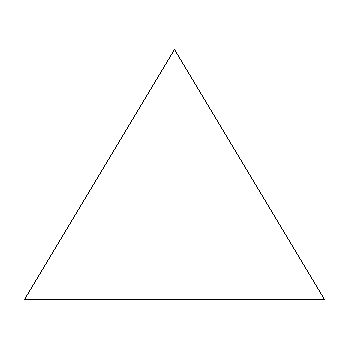
\includegraphics[width = 1in]{triangle}}\\
    \subfloat[Star]{\label{fig:star}
\includegraphics[width = 1in]{star}}
    \subfloat[House]{\label{fig:house}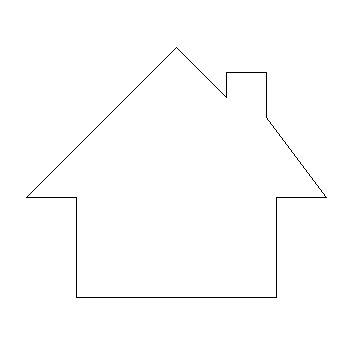
\includegraphics[width = 1in]{house}}
    \subfloat[Square Path]{\label{fig:sqpath}
\includegraphics[width = 1in]{squarePath}}\\
 \end{center}
  \caption{Multiple figure insertion example}
  \label{fig:testedShapes}
\end{figure}

\subsection{Using Tables}
Tables can be entered directly into your LaTeX document; however, inserting tables directly into your dissertation .tex file can result in unwanted clutter. It is generally cleaner to write the table in its own .tex file and then insert the .tex file into your dissertation .tex file. This is the method used by this template. An example table can be seen in Table \ref{table:test}.


\begin{table}
\scriptsize
\renewcommand{\tabcolsep}{0.09cm}
\centering
% Table generated by Excel2LaTeX from sheet 'Sheet1'
\begin{tabular}{rrcc}
\addlinespace
\toprule
\multicolumn{ 2}{c}{{\bf Condition}} & {\bf Metric I} & {\bf Metric II} \\
\otoprule
{\bf } & {\bf Mean} & 1505.644 & 1428.076 \\
{\bf Method A} & {\bf Std} & 726.160 & 541.098 \\
{\bf } & {\bf Reduction} & 0.000 & 0.000 \\
\midrule
{\bf } & {\bf Mean} & 1490.841 & 1426.620 \\
{\bf Method B} & {\bf Std} & 735.995 & 543.489 \\
{\bf } & {\bf Reduction} & 14.803 & 1.456 \\
\midrule
{\bf } & {\bf Mean} & 591.843 & 458.001 \\
{\bf Method C} & {\bf Std} & 458.332 & 153.099 \\
{\bf } & {\bf Reduction} & 913.801 & 970.075 \\
\midrule
{\bf } & {\bf Mean} & 566.089 & 638.568 \\
{\bf Method D} & {\bf Std} & 701.194 & 304.485 \\
{\bf } & {\bf Reduction} & 939.555 & 789.508 \\
\midrule
{\bf } & {\bf Mean} & 242.422 & 186.369 \\
{\bf Method E} & {\bf Std} & 390.052 & 129.654 \\
      & {\bf Reduction} & 1263.222 & 1241.707 \\
\midrule
\end{tabular}

\caption{A sample table.}
\label{table:test}
\end{table}




\subsection{Equations and Equation Arrays}
A simple equation can be seen in Equation \ref{eqn:slope}:
\begin{equation}
\centering
m = \frac{y_{2} - y_{1}}{x_{2} - x_{1}}.
\label{eqn:slope}
\end{equation}

An equation array can be seen in Equation \ref{eqn:generalBez}: 

\begin{eqnarray}
\lefteqn{B(t) =  \sum_{i=0}^n \binom{n}{i} (1-t)^{n-i}t^{i}\mathbf{P}_i }\nonumber \\ 
& = & (1-t)^{n}\mathbf{P}_0 + \binom{n}{1}t\mathbf{P}_1+ \cdots  \nonumber \\
 &\cdots & + \binom{n}{n-1}(1-t)^{n-1}\mathbf{P}_{n-1} + t^{n}\mathbf{P}_n, \phantom{ttt} t \in [0,1]
\label{eqn:generalBez}
\end{eqnarray}

\subsection{Algorithms}
An example of a Bayes' Filter \citep*{Thrun2005} algorithm can be seen in Algorithm \ref{alg:bayes}. Note that there are numerous methods for inserting algorithms. This template just demonstrates one.

\begin{algorithm}{$\mathbf{Bayes Filter}$}[$bel(x_{t-1})$, $u_t$, $z_t$]
\caption{The Bayes filter algorithm.}
\label{alg:bayes}
\begin{algorithmic}[1]
\FOR{all $x_t$}
\STATE $\overline{bel}(x_t) = \int p(x_t | u_t, x_{t-1}) bel(x_{t-1})dx_{t-1}$
\STATE $bel(x_t) = \eta p(z_t | x_t) \overline{bel}(x_t)$
\ENDFOR
\RETURN $bel(x_t)$
\end{algorithmic}
\end{algorithm}



\chapter{Other Important Dissertation Topics}
This chapter will discuss briefly other topics important to dissertation completion. Specifically, how to handle lists of figures and tables, as well as how to generate acronyms/abbreviations. Inserting references will also be discussed.

\section{ Lists of Figures, Tables, and Acronyms}
Lists of figures and tables should be built automatically from the figures and tables you insert in this document. The list of acronyms is also generated automatically, but acronyms must be defined before they can be added to a list of acronyms. See the \nomenclature{VDF}{Vanderbilt Dissertation Format} VanderbiltDissertationFormat.tex (VDF) file for an example of how to insert an acronym appropriately. Note that there are numerous ways within LaTeX to manage lists of acronyms. This template utilizes the nomencl package.

\section{Using References}
There are numerous methods to insert references into your document. Please refer to the VanderbiltDissertationFormat.tex file to see how references were added to this document and how the Bibliography was generated.